%% ****** Start of file apstemplate.tex ****** %
%%
%%
%%   This file is part of the APS files in the REVTeX 4 distribution.
%%   Version 4.1r of REVTeX, August 2010
%%
%%
%%   Copyright (c) 2001, 2009, 2010 The American Physical Society.
%%
%%   See the REVTeX 4 README file for restrictions and more information.
%%
%
% This is a template for producing manuscripts for use with REVTEX 4.0
% Copy this file to another name and then work on that file.
% That way, you always have this original template file to use.
%
% Group addresses by affiliation; use superscriptaddress for long
% author lists, or if there are many overlapping affiliations.
% For Phys. Rev. appearance, change preprint to twocolumn.
% Choose pra, prb, prc, prd, pre, prl, prstab, prstper, or rmp for journal
%  Add 'draft' option to mark overfull boxes with black boxes
%  Add 'showpacs' option to make PACS codes appear
%  Add 'showkeys' option to make keywords appear
%\documentclass[aps,prl,twocolumn,groupedaddress]{revtex4-1}
\documentclass[%
%reprint,
%superscriptaddress,
%groupedaddress,
%unsortedaddress,
%runinaddress,
%frontmatterverbose, 
twocolumn,
showpacs,preprintnumbers,
%nofootinbib,
%nobibnotes,
%bibnotes,
% amsmath,
 %amssymb,
 aps,
%pra,
%prb,
%rmp,
prstab,
%prstper,
%floatfix,
]{revtex4-1}
%\documentclass[aps,prl,preprint,superscriptaddress]{revtex4-1}
%\documentclass[aps,prl,reprint,groupedaddress]{revtex4-1}

% You should use BibTeX and apsrev.bst for references
% Choosing a journal automatically selects the correct APS
% BibTeX style file (bst file), so only uncomment the line
% below if necessary.
%\bibliographystyle{apsrev4-1}


\usepackage{graphics} % for pdf, bitmapped graphics files
\usepackage[pdftex]{graphicx}
\usepackage{epstopdf}
\usepackage[cmex10]{amsmath}
%\interdisplaylinepenalty=2500
\usepackage{amssymb}  % assumes amsmath package installed
%\usepackage{enumerate}
%\usepackage{setspace}
%\usepackage{verbatim}
\usepackage[colorlinks,linkcolor=blue,pdfauthor=Spencer \ Gessner,citecolor=red]{hyperref}
%\usepackage{hyperref}

\newcommand{\AFFslac}{\affiliation{SLAC National Accelerator Laboratory, Menlo Park, CA 94025, USA}}
\newcommand{\AFFucla}{\affiliation{University of California Los Angeles, Los Angeles, CA 90095, USA}}
\newcommand{\AFFoslo}{\affiliation{Department of Physics, University of Oslo, 0316 Oslo, Norway}}

\newtheorem{example}{Example}
\newtheorem{theorem}{Theorem}
\newtheorem{lemma}{Lemma}
\newtheorem{remark}{Remark}
\newtheorem{note}{Note}
\newtheorem{proof}{Proof}

\newtheorem{proposition}{Proposition}
\newtheorem{definition}{Definition}%{definition}
\newtheorem{assumption}{Assumption}
\newtheorem{corollary}{Corollary}%[section]

\begin{document}

% Use the \preprint command to place your local institutional report
% number in the upper righthand corner of the title page in preprint mode.
% Multiple \preprint commands are allowed.
% Use the 'preprintnumbers' class option to override journal defaults
% to display numbers if necessary
%\preprint{}

%Title of paper
\title{Longitudinal Phase Space Evolution and Tomographic Reconstruction at FACET}

% repeat the \author .. \affiliation  etc. as needed
% \email, \thanks, \homepage, \altaffiliation all apply to the current
% author. Explanatory text should go in the []'s, actual e-mail
% address or url should go in the {}'s for \email and \homepage.
% Please use the appropriate macro foreach each type of information

% \affiliation command applies to all authors since the last
% \affiliation command. The \affiliation command should follow the
% other information
% \affiliation can be followed by \email, \homepage, \thanks as well.
%\author{Spencer~Gessner}
\author{S.~Gessner}
\AFFslac

%%%%%%%%%%%%%%%%%%%%%%%%%%%%%%%%%%%%%%%
% All Other Authors (alphabetical)
\author{E.~Adli}
\AFFslac
\author{C.I.~Clarke}
\AFFslac
\author{S.~Corde}
\AFFslac
\author{F.J.~Decker}
\AFFslac
\author{A.S.~Fisher}
\AFFslac
\author{J.~Frederico}
\AFFslac
\author{M.J.~Hogan}
\AFFslac
\author{N.~Lipkowitz}
\AFFslac
\author{S.~Li}
\AFFslac
\author{M.~Litos}
\AFFslac
\author{D.~Walz}
\AFFslac
\author{G.~White}
\AFFslac
\author{V.~Yakimenko}
\AFFslac
\author{G.~Yocky}
\AFFslac

\email[]{sgess@slac.stanford.edu}
\thanks{This research was supported by DOE.}
%\affiliation{SLAC National Laboratory}

%Collaboration name if desired (requires use of superscriptaddress
%option in \documentclass). \noaffiliation is required (may also be
%used with the \author command).
%\collaboration can be followed by \email, \homepage, \thanks as well.
%\collaboration{}
%\noaffiliation

\date{\today}

\begin{abstract}
The Facility for Advanced Accelerator Experimental Tests (FACET) at SLAC produces high energy electron beams for Plasma Wakefield Acceleration (PWFA). PWFA experiments require high charge, high peak-current bunches in order to drive large amplitude wakes in the plasma. Creating short bunches with high charge requires detailed knowledge and control of the longitudinal phase space as it evolves in the linac. In this paper, we provide an overview of the bunch compression scheme at FACET and describe a novel tomographic method that allows us reconstruct the beam's longitudinal phase space at the end of the linac.
\end{abstract}

% insert suggested PACS numbers in braces on next line
%\pacs{41.85.Lc, 02.30.Yy, 29.20.-c, 02.60.-x}
% insert suggested keywords - APS authors don't need to do this
%\keywords{}

%\maketitle must follow title, authors, abstract, \pacs, and \keywords
\maketitle





%%%%%%%%%%%%%%%%%%%%%%%%%%%%%%%%%%%%%%%%%%%%%%%%%%%%%%%%%%%%%%%%%%%%%%%%%%%%%%%%%%%%%%%%

%%%%%%%%%%%%%%%%%%%%%%%%%%%%%%%%%%%%%%%%%%%%%%%%%%%%%%%%%%%%%%%%%%%%%%%%%%%%%%%%%%%%%%%%

\section{Introduction}
The Facility for Advanced Accelerator Experimental Tests (FACET) at SLAC produces high energy electron beams for Plasma Wakefield Acceleration (PWFA)~\cite{mjh_facet}. PWFA experiments require high charge, high peak-current bunches in order to drive large amplitude wakes in the plasma. Creating short bunches with high charge requires detailed knowledge and control of the longitudinal phase space as it evolves in the linac. In this paper, we provide a detailed description of the bunch compression scheme at FACET and describe a novel diagnostic for reconstructing the longitudinal phase space at the end of the linac.

FACET combines RF and wakefield chirping mechanisms with bunch compressor chicanes to generate the shortest bunches possible.

The 2D longitudinal particle tracking code LiTrack is used to supplement our understanding of the phase space in regions of the linac where diagnostics are not available.

The final bunch length is sensitive to many parameters in the linac, including initial bunch length, RF chirp phase, and the $R_{56}$ of compressor chicanes. To the greatest extent possible, feedbacks are implemented to control and stabilize the beam as it evolves in the linac. Some parameters are not under feedback control, and for this reason it is critical to have real time diagnostics for the bunch length, energy spectrum, and longitudinal phase space.

FACET uses an x-band transverse deflecting cavity (TCAV) for precision bunch length measurements and a half-period wiggler magnet for non-destructive energy spectrum measurements. These two diagnostics provide projections of the longitudinal phase space. A third measurement was developed by creating a tunable momentum aperture, or slit, and using the TCAV and spectrometer to diagnose mono-energetic slices of the beam. By combining the bunch profiles measured for each slice, we were able to tomographically reconstruct the beam's longitudinal phase space. The longitudinal phase space uniquely encodes the longitudinal evolution of the beam in the linac. This technique allows us to determine errors in linac parameters and is a valuable tool for beam tuning.

\begin{figure*}[htb]
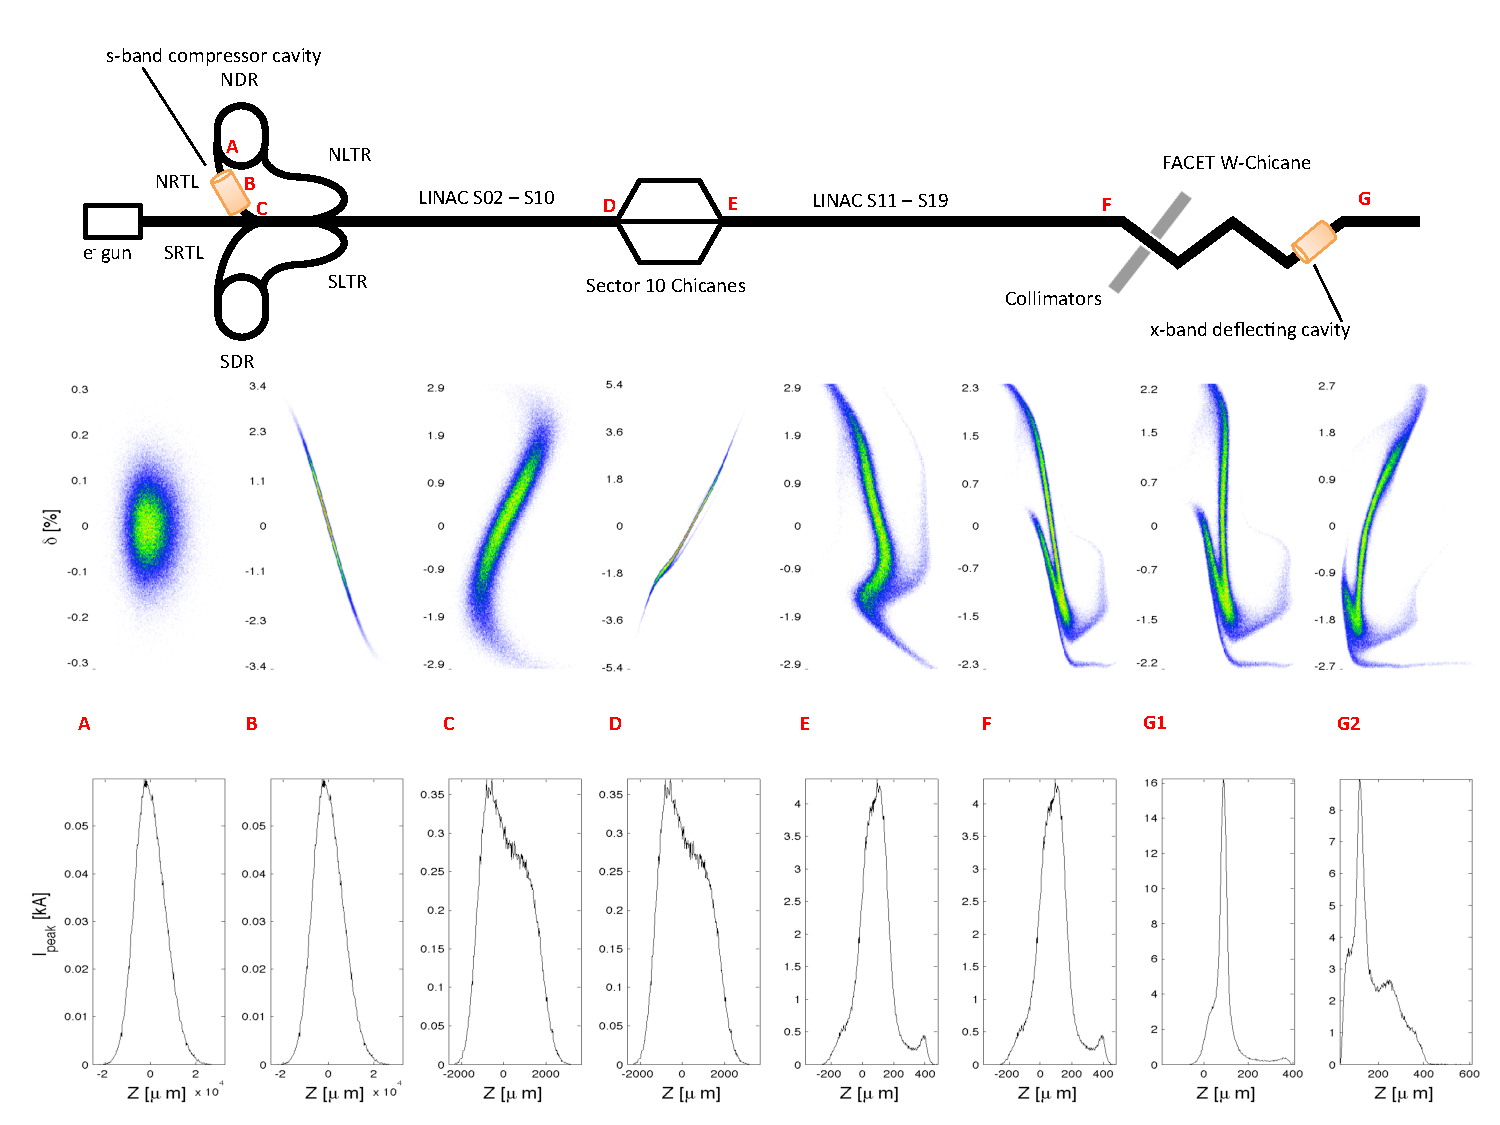
\includegraphics[width=\textwidth,height=12cm]{figures/facet_schem.pdf}
  \caption{Overview of the FACET Linac.}
  \label{schem}
\end{figure*}

%%%%%%%%%%%%%%%%%%%%%%%%%%%%%%%%%%%%%%%%%%%%%%%%%%%%%%%%%%%%%%%%%%%%%%%%%%%%%%%%%%%%%%%%

%%%%%%%%%%%%%%%%%%%%%%%%%%%%%%%%%%%%%%%%%%%%%%%%%%%%%%%%%%%%%%%%%%%%%%%%%%%%%%%%%%%%%%%%

\section{Longitudinal Phase Space Evolution}\label{sec:facet}

The electron beam is generated from a thermionic cathode and accelerated to 1.19 GeV before being transported to the North Damping Ring (NDR), shown on the left side of Figure~\ref{schem}. The bunch radiatively damps to an equilibrium bunch length and an equilibrium energy spread during the 16 ms store. We imaged synchrotron radiation generated by the beam in one of the bends with a Hamamatsu C5680 streak camera. The measured bunch length was $\sigma_z = 6.59$ mm, about 20\% longer than what was measured during SLC operation for similar bunch charge and RF parameters~\cite{Holtzapple}. Figure~\ref{streak} shows the streaked beam image for the final fives turns before extraction. The bunch is fit to an asymmetric gaussian with the form
\begin{equation}
 \lambda(z) = \frac{N_b}{\sqrt{2\pi}\sigma_z}\exp{ \left[-\frac{1}{2}\left(\frac{z}{(1\pm A)\sigma_z}\right)^2\right]}
\end{equation}
where $N_b$ is the number of beam electrons and $A$ is the asymmetry factor. The asymmetry arrises from the distortion of the RF potential due to beam loading.

\begin{figure}[htb]
  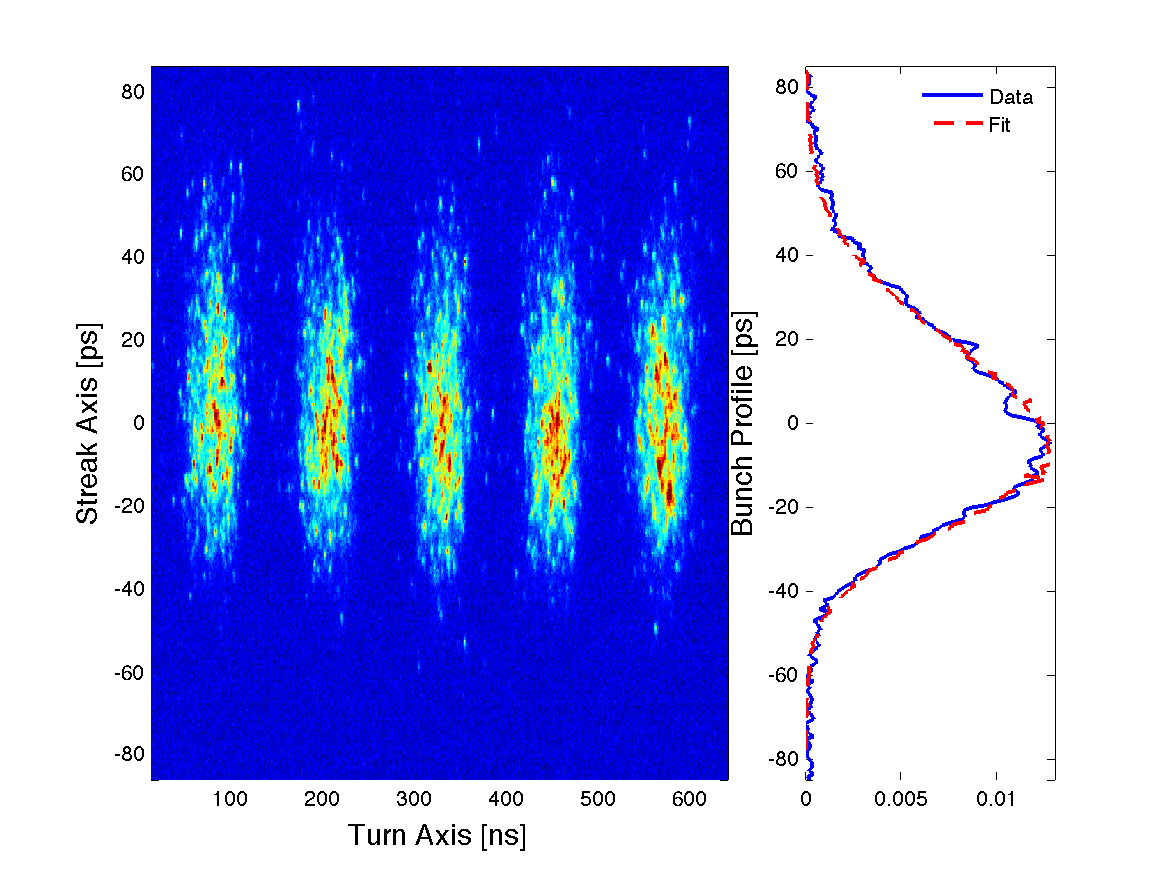
\includegraphics[width=\columnwidth]{figures/combo.pdf}
  \caption{Streak camera image of the final five turns before extraction from NDR. The bunch profile on the right is the average of the five turns shown, fit to an asymmetric gaussian with $\sigma_t = 22$ ps or $\sigma_z = 6.59$ mm, and asymmetry parameter -0.2.}
  \label{streak}
\end{figure}

The equilibrium energy spread is solely a function of the beam energy and lattice parameters and it is calculated to be $\sigma_{\delta} = 7.11 \times 10^{-4}$. There is no time-energy correlation of the beam in the ring, so the initial longitudinal phase space volume is given by $\varepsilon_{z0} = \sigma_z \sigma_{\delta} = 5.57$ MeV$\cdot$mm. $\varepsilon_{z0}$ sets a lower limit on the final bunch length that can be achieved at the end of the linac.

Upon extraction from the NDR, the beam is chirped by an the s-band compressor cavity. The beam is compressed by a factor of 10 in the North Ring to Linac (NRTL) chicane and enters the Linac with a 600 $\mu$m RMS bunch length. The bunch is slightly over-compressed, with a residual low-to-high chirp, so as to minimize the impact of wakefields in the linac. The bunch is accelerated in the first kilometer of the linac with a net phase of -20 degrees with respect to the crest (in SLAC coordinates, negative angles are ahead of crest). FACET uses a unique chirping scheme in the front end of the linac that staggers the phasing of the beam over nine linac sectors. The staggered chirp process is depicted in Figure~\ref{stag}. By accelerating on crest or nearly on crest in the first few sectors, the beam becomes stiff and more resistant to emittance dilution from transverse wakefields. The later sectors have stronger phasing, up to -55 degrees off crest, in order to achieve an average of -20 degrees chirp prior to the Sector 10 Chicane. While this scheme has the advantage of reducing emittance growth, it makes the beam more sensitive to phase errors in the highly chirped sectors.

\begin{figure}[hb]
  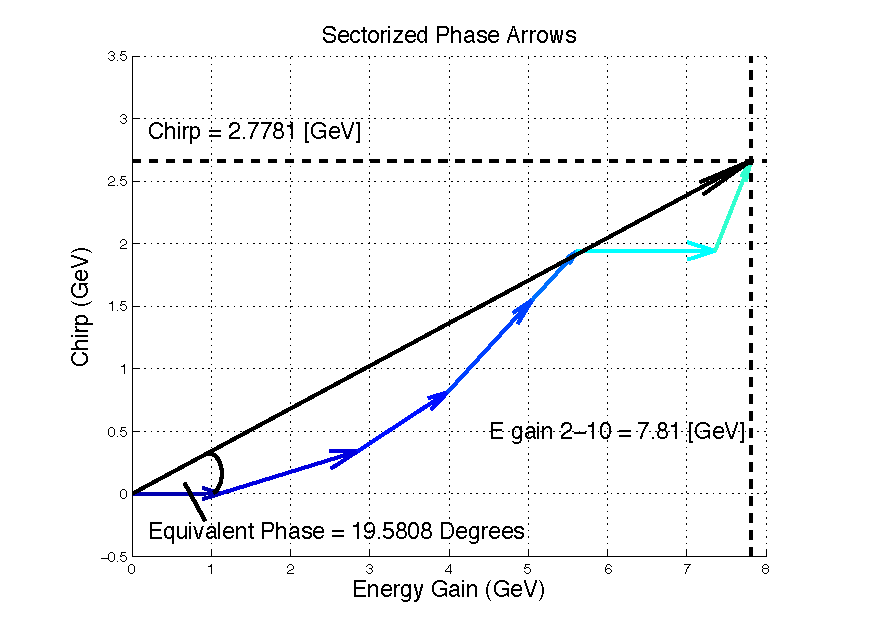
\includegraphics[width=\columnwidth]{figures/stag.pdf}
  \caption{Diagram showing the phasing in sectors 2-10 at FACET. Each arrow represents the phase and amplitude of the accelerating sector. Note that the chirping angle is depicted as a positive value for clarity.}
  \label{stag}
\end{figure}

The bunch is compressed by another factor of 10 in the Sector 10 Chicane. Again, the bunch is over-compressed, this time with a residual high-to-low chirp. The very short (50 $\mu$m), very high charge (3.2 nC) bunch drives a high-amplitude longitudinal wakefield in the SLAC s-band cavities. The wakeloss function $W(z)$ is a convolution of the cavity wake structure and the bunch profile, but for very short bunches it is roughly linear over the core of the bunch. The net effect of the wakefields in the second kilometer of the linac is to provide a mostly linear high-to-low chirp that will be leveraged for bunch compression in the FACET W-Chicane.

The FACET W-Chicane is a unique lattice that features adjustable $R_{56}$.  When extremely short bunches are needed, the chicane is tuned to $R_{56} = 5$ mm and yields a gaussian bunch with $\sigma_z = 20~\mu$m. For the two-bunch setup, the $R_{56} = 10$ mm, which over-compresses the bunch with a residual low-to-high chirp. Table~\ref{dat_table} lists 

\begin{table}
  \begin{tabular}{ l c c c}
    \hline
    Element & $R_{56}$ [mm] & $\phi_{rf}$ & $\sigma_z$ [$\mu$m] \\ \hline
    NDR &  & & 6600 \\
    NRTL Cavity &  & $ 90^o$ & 6600 \\
    NRTL Chicane & 602.6 & & 500 \\
    S02-10 &  & $-20^o$ & 500 \\
    S10 Chicane & -75.8 & & 50 \\
    S11-19 & & $0^o$ & 50 \\
    W-Chicane & 5,10 & & 20,200 \\
    \hline
  \end{tabular}
   \caption{Table of linac parameters and bunch lengths for each linac element. We quote the two $R_{56}$ values typically used in the W-Chicane.}
   \label{dat_table}
\end{table}

%In this case, the uncollimated bunch is non-gaussian with an RMS of 100-200 $\mu$m. A thin tantalum blade, referred to as the notch collimator, is inserted into the beam at a point where the ratio $\eta \delta / \sqrt{ \beta \varepsilon}$ is maximized early in the chicane. The notch collimator removes charge from the core of the energy spectrum, which corresponds to center of the bunch profile as a result of the $z-\delta$ correlation. Jaw collimators are used to remove high and low energy tails that lack $z-\delta$ correlation. This improves the final contrast of the two-bunch longitudinal profile.



%\begin{figure}[hbt]
%  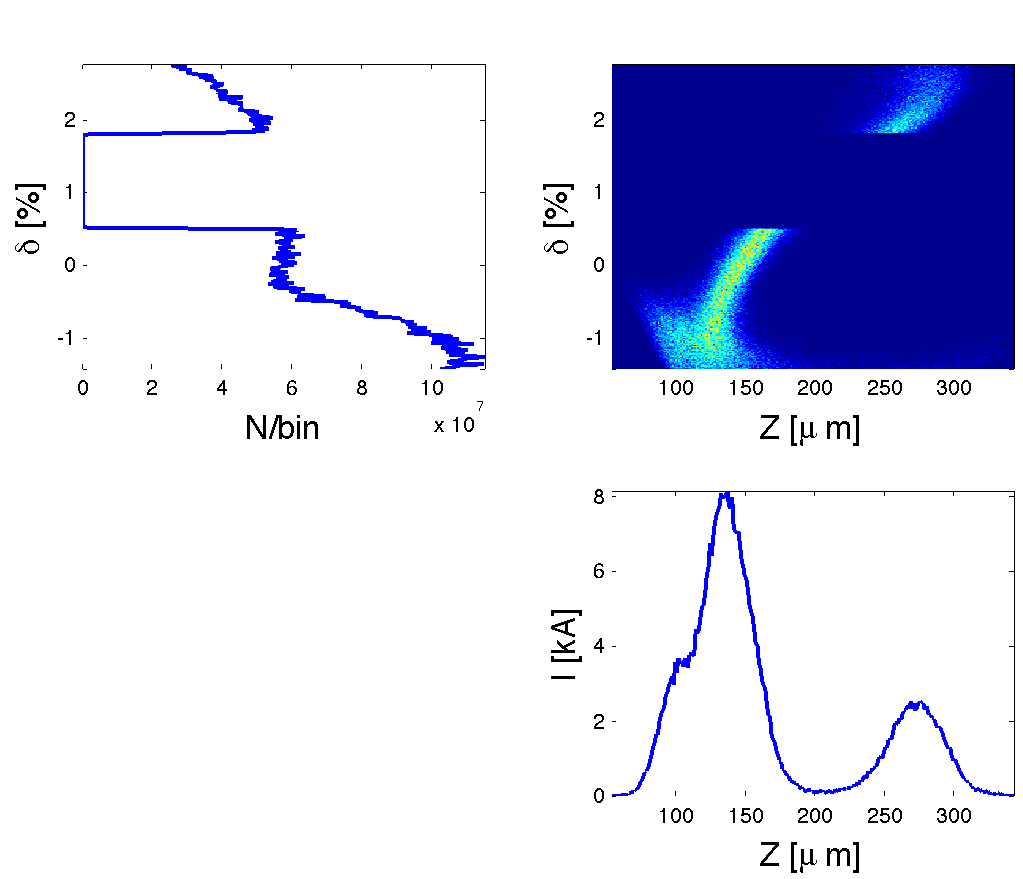
\includegraphics[width=\columnwidth]{figures/sect20.pdf}
%  \caption{LiTrack simulation of the longitudinal phase space after collimation and compression in the W-Chicane.}
%  \label{sect20}
%\end{figure}

%%%%%%%%%%%%%%%%%%%%%%%%%%%%%%%%%%%%%%%%%%%%%%%%%%%%%%%%%%%%%%%%%%%%%%%%%%%%%%%%%%%%%%%%

%%%%%%%%%%%%%%%%%%%%%%%%%%%%%%%%%%%%%%%%%%%%%%%%%%%%%%%%%%%%%%%%%%%%%%%%%%%%%%%%%%%%%%%%

\section{Diagnostics}\label{sec:diag}
A transverse deflecting x-band cavity (TCAV) is located near the end of the W-Chicane, close to maxima in $\beta_y$. The TCAV is used as a vertical streaking device; electrons with different longitudinal positions $z$ in a bunch experience different transverse deflecting fields. The particles are displaced vertically according to
\begin{equation}
\Delta Y = R_{34}\frac{e V_{rf}}{E_0}\sin{kz}
\end{equation}
and $R_{34}$ is the matrix element between the TCAV and the location where the streaked beam is imaged on a screen. The TCAV phase is calibrated such that the position $z=0$ in the beam corresponds to the zero crossing of the deflecting wave. The TCAV is the only diagnostic that has been used experimentally to resolve femtosecond beam structures. However, the TCAV is a destructive diagnostic, so it is not used while taking experimental data with plasma.

A half-period wiggler magnet is located just downstream of the TCAV at a dispersive point with the same $\eta$ and $\beta$ as the notch collimator. The wiggler deflects the horizontally-dispersed beam vertically. This generates a streak of synchrotron x-rays which are intercepted by a scintillating YAG:Ce crystal millimeters above the beam path. The x-ray streak encodes the energy spectrum of the beam onto the crystal, which is imaged by a CCD camera. On average, each 20.35 GeV electron radiates away 67 KeV of x-rays Emittance dilution due to ISR and CSR is negligible, so we the wiggler/YAG energy spectrometer is non-destructive. This is a particularly useful diagnostic, because it provides information about the longitudinal phase space on every shot.

\section{Tomographic Phase Space Reconstruction}\label{sec:tomo}
An ideal phase space measurement projects the beam's longitudinal profile and energy spectrum into the $XY$ plane so that the phase space can be imaged optically. For instance, the LCLS TCAV streaks the beam horizontally before the beam passes through a vertical dipole. The beam is imaged at a point of large $R_{36}$ and large $R_{15}$ so that the entire longitudinal phase space is resolved on every shot. 

At FACET, it is not possible to streak and disperse the beam in orthogonal planes without significant changes to the chicane and final focus optics. Instead, we have developed a technique that allows us to tomographically reconstruct the beam's longitudinal phase space.  We use the jaw collimators at the beginning of the FACET chicane to create a narrow slit and use the TCAV to streak the portion of the beam that passes through the slit. The collimators are located in a region with good dispersive contrast, where the ratio $\eta \delta / \sqrt{\beta \varepsilon}$ is at a maximum, so the slit acts as a momentum aperture. The collimators are moved across the path of the dispersed beam while maintaining a constant slit width of roughly 180 $\mu$m or $\Delta E/E = 0.25\%$. The total energy spread of the beam is 2.5\% FWHM. Figure~\ref{slit} shows the measured energy spectrum of the beam with the collimators open and with the slit in place.

\begin{figure}[hbt]
  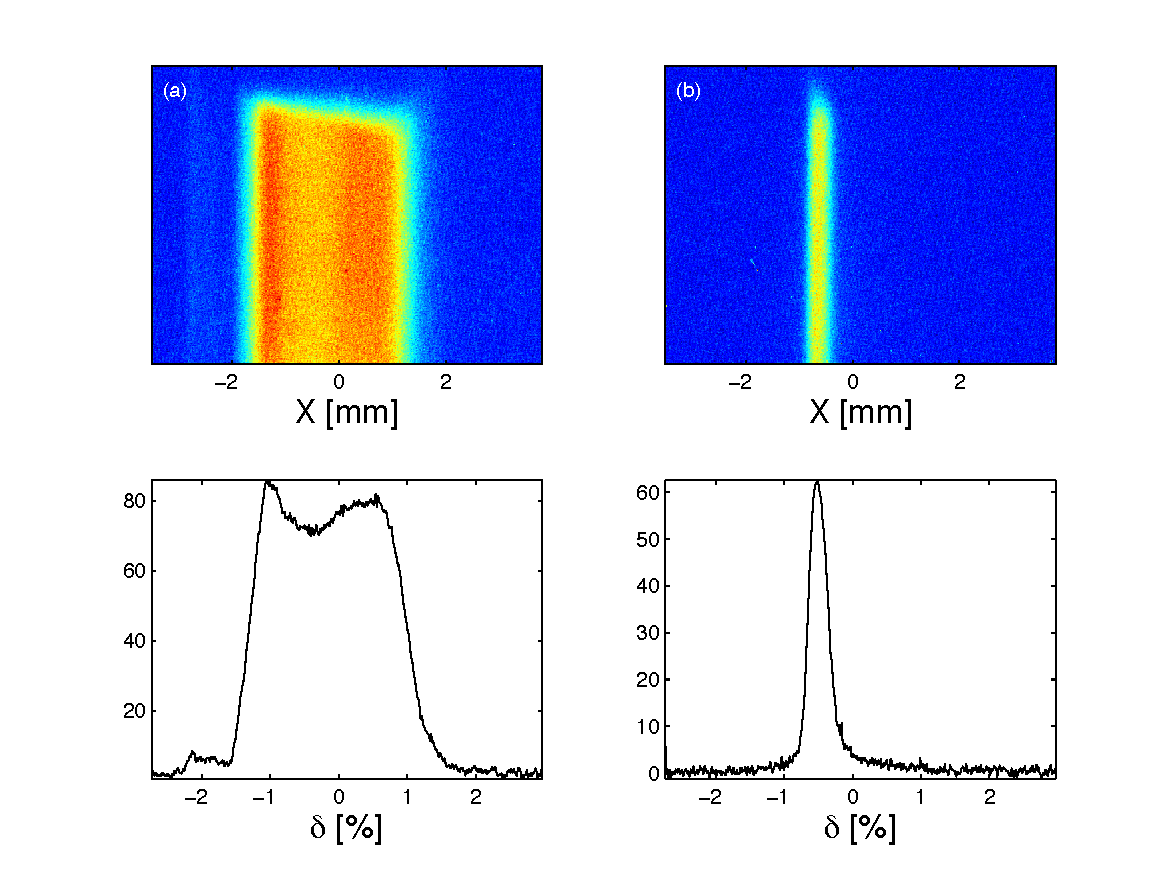
\includegraphics[width=\columnwidth]{figures/slit_wlabel.pdf}
  \caption{(a) The full beam energy spectrum imaged at the wiggler spectrometer. (b) The partial energy spectrum with the slit acting as a momentum aperture. The dispersion was measured to be 128 mm at this location.}
  \label{slit}
\end{figure}

The longitudinal bunch profile is recorded for each position of the slit. Figure~\ref{tcav_slit} shows the measured bunch profiles with the collimators open and with the slit in place.

\begin{figure}[hbt]
  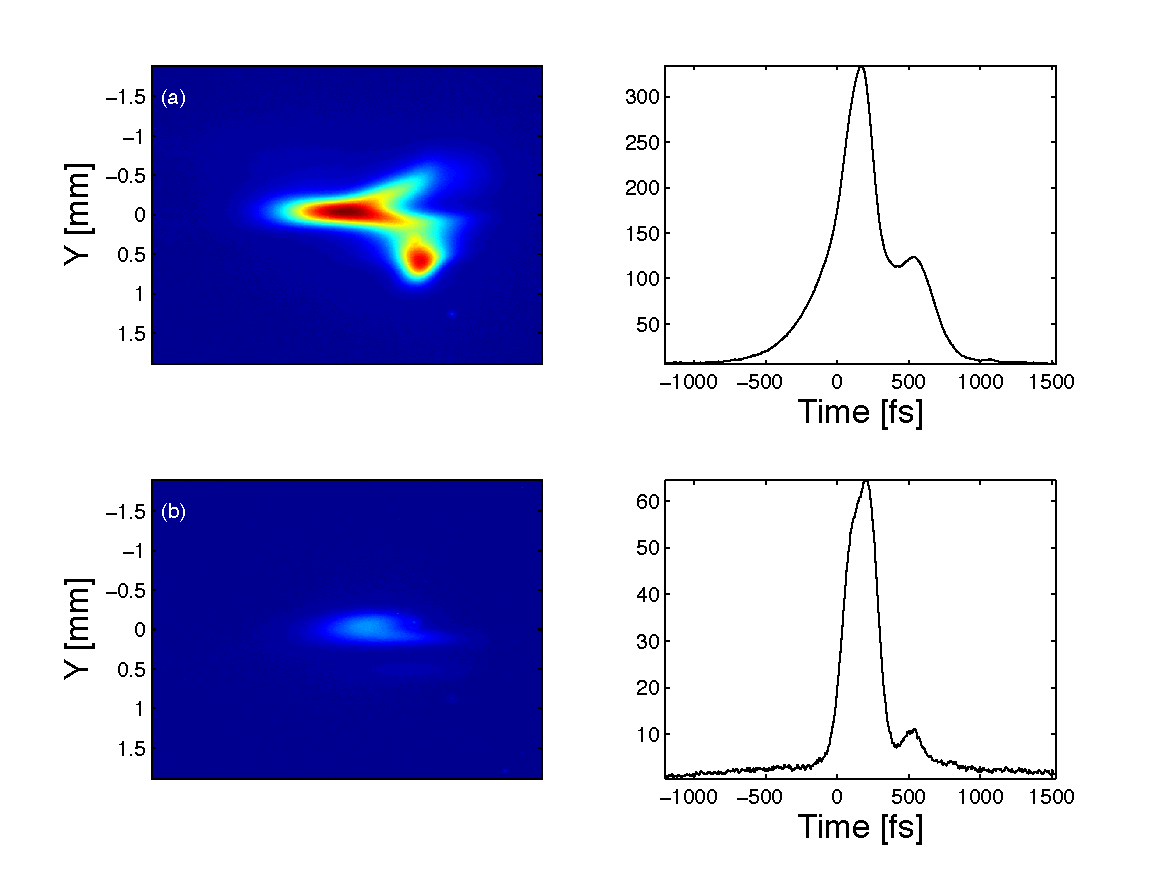
\includegraphics[width=\columnwidth]{figures/tcav_slit2.pdf}
  \caption{(a) The full bunch profile as measured with the TCAV. (b) The bunch profile measured for a monoenergetic beam slice.}
  \label{tcav_slit}
\end{figure}

Figure~\ref{raw_data} shows the profiles from a measurement taken for 10 slit positions with 20 shots each. Each profile is stackedThere is an inherent arrival time jitter of the beam relative to the RF phase of the TCAV with an RMS of roughly 250 fs. To correct for jitter, we locate the maximum value of each profile and calculate the average position of the maximum for each set of 20 shots. The shots are aligned to the average position

\begin{figure}[hbt]
  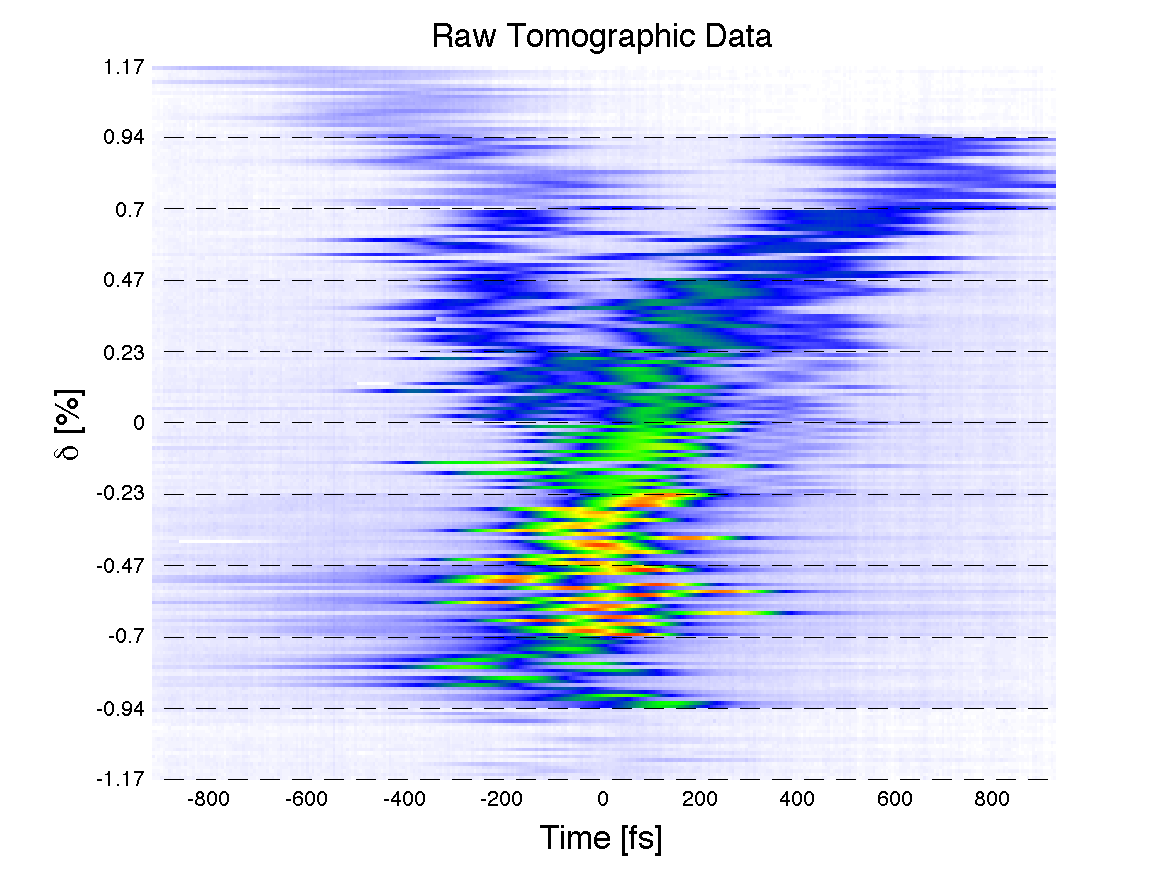
\includegraphics[width=\columnwidth]{figures/raw.pdf}
  \caption{Raw data from the tomographic slit scan measurement. Note that the $\delta$ axis is not continuous. The dashed black lines denote consecutive shots for each slit position.}
  \label{raw_data}
\end{figure}

\begin{figure}[hbt]
  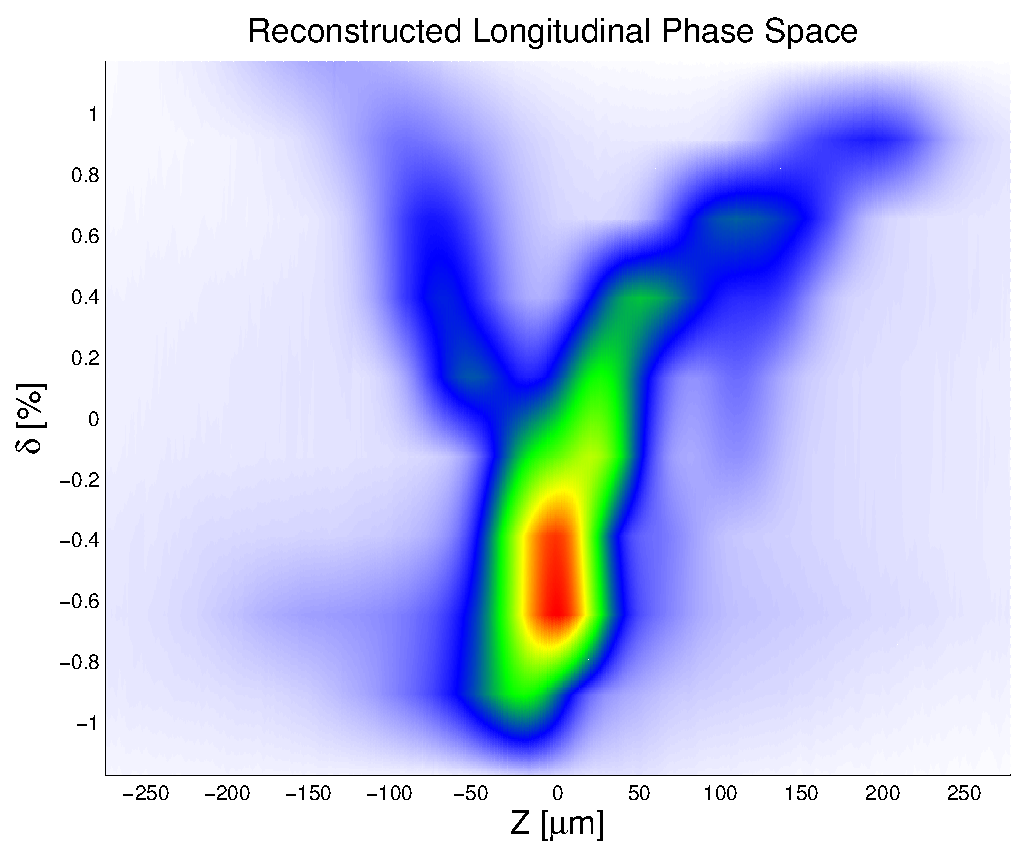
\includegraphics[width=\columnwidth]{figures/test.pdf}
  \caption{Raw data from the tomographic slit scan measurement.}
  \label{ps}
\end{figure}




\section{Conclusions and Future Work} \label{sec:con}


xxxxxxxxx


%%%%%%%%%%%%%%%%%%%%%%%%%%%%%%%%%%%%%%%%%%%%%%%%%%%%%%%%%%%%%%%%%%%%%%%%%%%%%%%%%%%%%%%%

%%%%%%%%%%%%%%%%%%%%%%%%%%%%%%%%%%%%%%%%%%%%%%%%%%%%%%%%%%%%%%%%%%%%%%%%%%%%%%%%%%%%%%%%



\begin{thebibliography}{99}

\bibitem{mjh_facet} M. J. Hogan et al., New J. Phys. 12, 055030 (2010).

\bibitem{Holtzapple} R. Holtzapple, Ph.D. Thesis, Stanford University (1996).

\end{thebibliography}


\end{document}


